\documentclass[aspectratio=169,11pt]{beamer}
\usetheme{moloch}

\usepackage[T1]{fontenc}
\usepackage{booktabs}
\usepackage{pgfplots}
\pgfplotsset{compat=1.18}
\usetikzlibrary{positioning,arrows.meta,shapes.misc,fit,calc}

% palette
\definecolor{keep}{HTML}{2A6F97}     % models we keep
\definecolor{modern}{HTML}{E07A1F}   % modern replacement / new
\definecolor{dropc}{HTML}{BDBDBD}    % not in our study
\definecolor{p20}{HTML}{A9CCE3}
\definecolor{p50}{HTML}{5499C7}
\definecolor{p80}{HTML}{1F4E79}
\newcommand{\hl}[1]{\textbf{\color{modern}#1}}

\tikzset{
  box/.style={draw=keep, fill=keep!8, rounded corners=3pt, align=center,
              font=\scriptsize, minimum height=9mm, inner sep=3pt},
  hbox/.style={box, draw=modern, fill=modern!10},
  arr/.style={-{Stealth[length=2mm]}, thick, draw=black!60},
}

\title{Supervised Learning Algorithms, 20 Years Later}
\subtitle{Replicating Caruana \& Niculescu-Mizil (ICML 2006) on GPUs --- Experiment Design}
\author{Tom Taylor}
\institute{COGS 118A Final Project \quad$\cdot$\quad November 2026}
\date{}

\begin{document}

% ================================================================ 1
\maketitle

% ================================================================ 2
\begin{frame}{The 2006 Result and What We Change}
\begin{columns}[T]
\begin{column}{0.53\textwidth}
\centering
{\scriptsize\textbf{Paper's ranking} (best variant per model, Table 2)}\\[2pt]
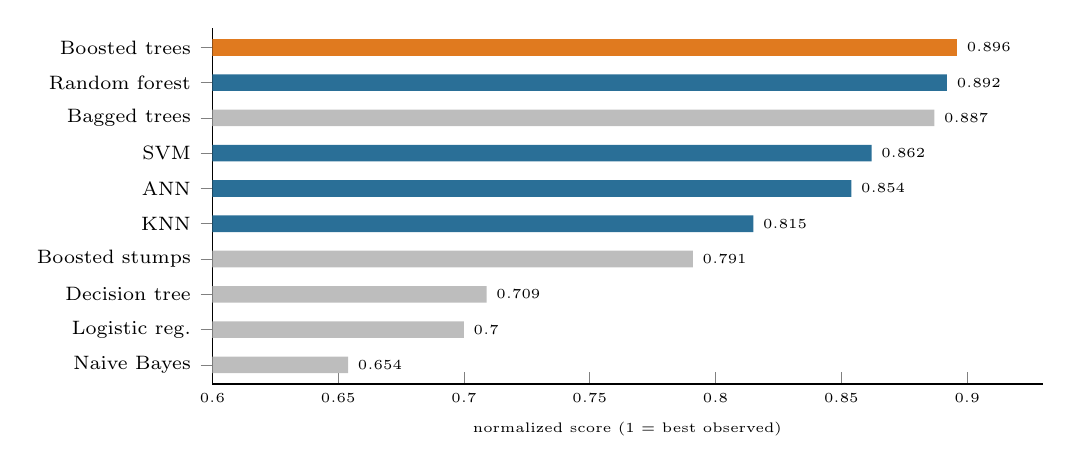
\begin{tikzpicture}
\begin{axis}[
  xbar, width=\linewidth, height=6.1cm,
  xmin=0.6, xmax=0.93, bar width=6pt,
  y dir=reverse, bar shift=0pt,
  ytick={Boosted trees,Random forest,Bagged trees,SVM,ANN,KNN,Boosted stumps,Decision tree,Logistic reg.,Naive Bayes},
  symbolic y coords={Boosted trees,Random forest,Bagged trees,SVM,ANN,KNN,Boosted stumps,Decision tree,Logistic reg.,Naive Bayes},
  yticklabel style={font=\scriptsize}, xticklabel style={font=\tiny},
  nodes near coords, nodes near coords style={font=\tiny, /pgf/number format/.cd, fixed, precision=3},
  axis x line*=bottom, axis y line*=left, enlarge y limits=0.06,
  xlabel={\tiny normalized score (1 = best observed)},
]
\addplot[fill=modern, draw=none] coordinates {(0.896,Boosted trees)};
\addplot[fill=keep, draw=none] coordinates {(0.892,Random forest) (0.862,SVM) (0.854,ANN) (0.815,KNN)};
\addplot[fill=dropc, draw=none] coordinates {(0.887,Bagged trees) (0.791,Boosted stumps) (0.709,Decision tree) (0.700,Logistic reg.) (0.654,Naive Bayes)};
\end{axis}
\end{tikzpicture}\\[-1pt]
{\tiny
\textcolor{keep}{\rule{6pt}{6pt}} kept \quad
\textcolor{modern}{\rule{6pt}{6pt}} kept as XGBoost \quad
\textcolor{dropc}{\rule{6pt}{6pt}} not in our study}
\end{column}
\begin{column}{0.44\textwidth}
\footnotesize
\textbf{What changes}
\begin{itemize}\scriptsize
  \item 6 models: 4 from the paper + \hl{XGBoost} + \hl{TabPFN}
  \item 4 datasets, up to \textbf{100k} rows (paper trained on 4k)
  \item Accuracy only (paper used 8 metrics)
  \item \hl{3 train sizes} (20/50/80\%) $\times$ 3 trials
  \item 5-fold \texttt{GridSearchCV} on T4-class GPUs
\end{itemize}
\medskip
\textbf{Questions}
\begin{enumerate}\scriptsize
  \item Does the 2006 ranking hold with up to 20$\times$ more training data?
  \item Do modern boosting and a tabular foundation model change it?
\end{enumerate}
\end{column}
\end{columns}
\end{frame}

% ================================================================ 3
\begin{frame}{How Much Data Each Model Sees}
\begin{columns}[T]
\begin{column}{0.6\textwidth}
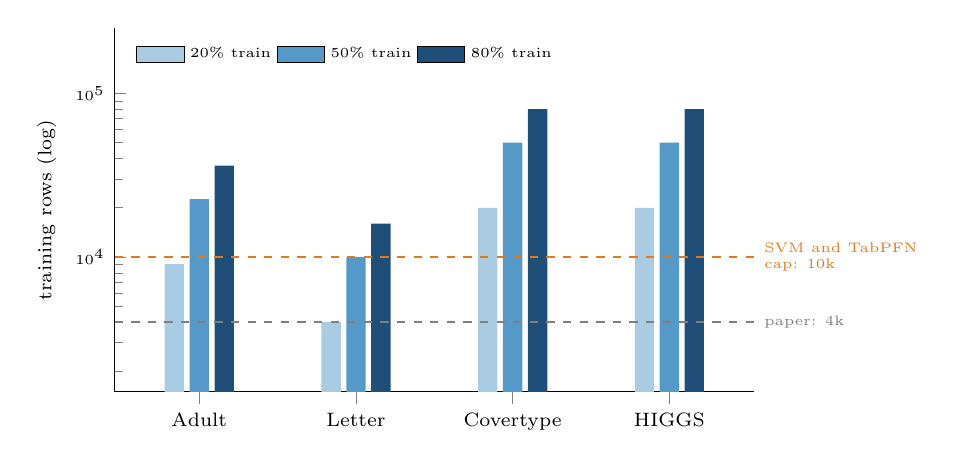
\begin{tikzpicture}
\begin{axis}[
  ybar, width=0.8\linewidth, height=6.2cm,
  ymode=log, log origin=infty, ymin=1500, ymax=2.5e5,
  bar width=7pt, enlarge x limits=0.18,
  symbolic x coords={Adult,Letter,Covertype,HIGGS}, xtick=data,
  xticklabel style={font=\scriptsize}, yticklabel style={font=\tiny},
  ylabel={\scriptsize training rows (log)},
  legend style={font=\tiny, at={(0.02,0.98)}, anchor=north west, legend columns=3, draw=none, fill=none},
  axis x line*=bottom, axis y line*=left, clip=false, area legend,
]
\addplot[fill=p20, draw=none] coordinates {(Adult,9044) (Letter,4000) (Covertype,20000) (HIGGS,20000)};
\addplot[fill=p50, draw=none] coordinates {(Adult,22611) (Letter,10000) (Covertype,50000) (HIGGS,50000)};
\addplot[fill=p80, draw=none] coordinates {(Adult,36177) (Letter,16000) (Covertype,80000) (HIGGS,80000)};
\legend{20\% train, 50\% train, 80\% train}
\draw[dashed, thick, gray] ({rel axis cs:0,0}|-{axis cs:Adult,4000}) -- ({rel axis cs:1,0}|-{axis cs:Adult,4000})
  node[pos=1, anchor=west, align=left, font=\tiny, gray] {paper: 4k};
\draw[dashed, thick, modern] ({rel axis cs:0,0}|-{axis cs:Adult,10000}) -- ({rel axis cs:1,0}|-{axis cs:Adult,10000})
  node[pos=1, anchor=west, align=left, font=\tiny, modern] {SVM and TabPFN\\cap: 10k};
\end{axis}
\end{tikzpicture}
\end{column}
\begin{column}{0.37\textwidth}
\scriptsize
\textbf{Datasets} (binary)\\[2pt]
\begin{tabular}{@{}lrr@{}}
\toprule
 & Feat. & \% pos \\
\midrule
Adult & 104 & 24.8 \\
Letter & 16 & 50.3 \\
Covertype & 54 & 48.8 \\
HIGGS & 28 & 53.0 \\
\bottomrule
\end{tabular}

\medskip
\textbf{Classifiers} (all GPU)\\[2pt]
\textcolor{keep}{\textbf{Paper:}} random forest, SVM (RBF), MLP, KNN (cuML, skorch)\\
\textcolor{modern}{\textbf{Modern:}} XGBoost, TabPFN v2 (no tuning)

\medskip
{\tiny Covertype and HIGGS: one 100k-row stratified subsample, shared by all models. Above the orange line, SVM and TabPFN train on a 10k subsample (same test set).}
\end{column}
\end{columns}
\end{frame}

% ================================================================ 4
\begin{frame}{Protocol: One Cell of the Experiment}
\centering
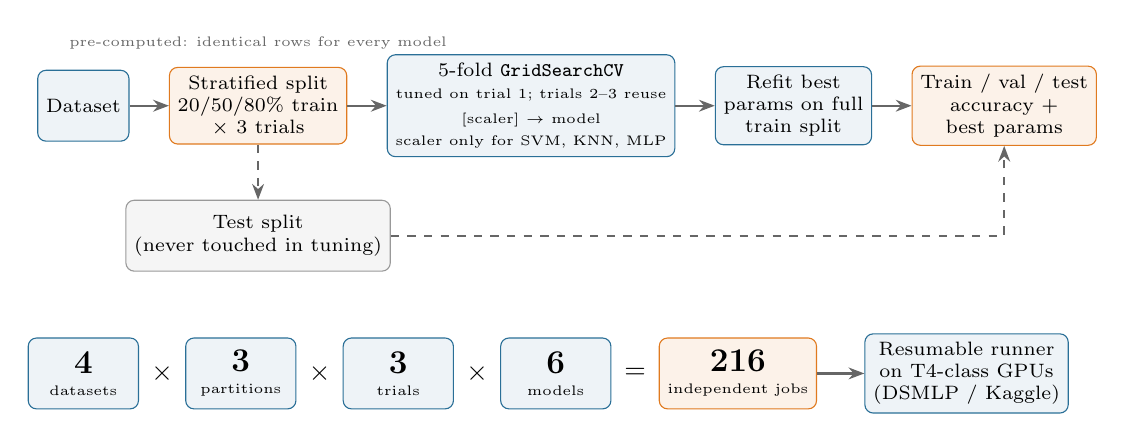
\begin{tikzpicture}[node distance=5mm]
  \node[box] (data) {Dataset};
  \node[hbox, right=of data] (split) {Stratified split\\20/50/80\% train\\$\times$ 3 trials};
  \node[box, right=of split, minimum width=34mm] (cv) {5-fold \texttt{GridSearchCV}\\{\tiny tuned on trial 1; trials 2--3 reuse}\\[1pt]
     {\tiny [scaler] $\rightarrow$ model}\\{\tiny scaler only for SVM, KNN, MLP}};
  \node[box, right=of cv] (refit) {Refit best\\params on full\\train split};
  \node[hbox, right=of refit] (out) {Train / val / test\\accuracy +\\best params};
  \draw[arr] (data) -- (split);
  \draw[arr] (split) -- (cv);
  \draw[arr] (cv) -- (refit);
  \draw[arr] (refit) -- (out);
  \node[box, draw=black!40, fill=black!4, below=7mm of split] (test) {Test split\\(never touched in tuning)};
  \draw[arr, dashed] (split) -- (test);
  \draw[arr, dashed] (test.east) -| (out.south);
  \node[font=\tiny, black!60, above=1mm of split] {pre-computed: identical rows for every model};

  % job grid
  \begin{scope}[yshift=-34mm]
    \foreach \lab/\n [count=\i] in {datasets/4, partitions/3, trials/3, models/6} {
      \node[box, minimum width=14mm] (g\i) at ({(\i-1)*20mm},0) {\textbf{\large \n}\\{\tiny \lab}};
    }
    \foreach \i in {1,2,3} { \node at ($(g\i.east)!0.5!(g\the\numexpr\i+1\relax.west)$) {$\times$}; }
    \node[hbox, right=6mm of g4, minimum width=16mm] (jobs) {\textbf{\large 216}\\{\tiny independent jobs}};
    \node at ($(g4.east)!0.5!(jobs.west)$) {$=$};
    \node[box, right=6mm of jobs] (gpu) {Resumable runner\\on T4-class GPUs\\(DSMLP / Kaggle)};
    \draw[arr] (jobs) -- (gpu);
  \end{scope}
\end{tikzpicture}

\vspace{4pt}
{\scriptsize Timing test first (HIGGS 100k, all models, 80/20, 1 trial) \,$\cdot$\, est.\ 5--10 GPU-hours \,$\cdot$\, RF \texttt{max\_depth} pinned}
\end{frame}

% ================================================================ 5
\begin{frame}{Planned Analyses \emph{(sketches, not results)}}
\centering
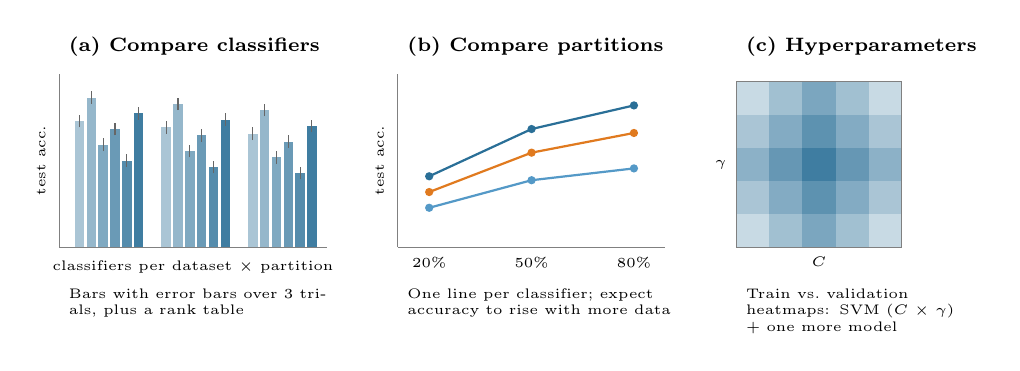
\begin{tikzpicture}
% (a) grouped bars
\begin{scope}
  \draw[black!50] (0,0) -- (3.4,0); \draw[black!50] (0,0) -- (0,2.2);
  \foreach \g in {0,1,2} {
    \foreach \h [count=\j] in {1.6,1.9,1.3,1.5,1.1,1.7} {
      \pgfmathsetmacro{\x}{0.2+\g*1.1+(\j-1)*0.15}
      \fill[keep!\the\numexpr 30+\j*10\relax] (\x,0) rectangle ++(0.12,\h-\g*0.08);
      \draw[black!60] (\x+0.06,\h-\g*0.08-0.08) -- ++(0,0.16);
    }
  }
  \node[font=\tiny, anchor=north] at (1.7,-0.05) {classifiers per dataset $\times$ partition};
  \node[font=\tiny, rotate=90, anchor=south] at (-0.05,1.1) {test acc.};
  \node[font=\scriptsize\bfseries, anchor=south west] at (0,2.3) {(a) Compare classifiers};
  \node[font=\tiny, align=left, anchor=north west, text width=3.4cm] at (0,-0.4) {Bars with error bars over 3 trials, plus a rank table};
\end{scope}
% (b) learning curves
\begin{scope}[xshift=4.3cm]
  \draw[black!50] (0,0) -- (3.4,0); \draw[black!50] (0,0) -- (0,2.2);
  \foreach \a/\b/\c/\col in {0.9/1.5/1.8/keep, 0.7/1.2/1.45/modern, 0.5/0.85/1.0/p50} {
    \draw[thick, \col] (0.4,\a) -- (1.7,\b) -- (3.0,\c);
    \foreach \x/\y in {0.4/\a,1.7/\b,3.0/\c} \fill[\col] (\x,\y) circle (1.5pt);
  }
  \foreach \x/\l in {0.4/20\%,1.7/50\%,3.0/80\%} \node[font=\tiny, anchor=north] at (\x,0) {\l};
  \node[font=\tiny, rotate=90, anchor=south] at (-0.05,1.1) {test acc.};
  \node[font=\scriptsize\bfseries, anchor=south west] at (0,2.3) {(b) Compare partitions};
  \node[font=\tiny, align=left, anchor=north west, text width=3.4cm] at (0,-0.4) {One line per classifier; expect accuracy to rise with more data};
\end{scope}
% (c) heatmap
\begin{scope}[xshift=8.6cm]
  \foreach \i in {0,...,4} { \foreach \j in {0,...,4} {
    \pgfmathtruncatemacro{\v}{max(10, 90 - 18*abs(\i-2) - 14*abs(\j-2))}
    \fill[keep!\v] (\i*0.42,\j*0.42) rectangle ++(0.42,0.42);
  }}
  \draw[black!50] (0,0) rectangle (2.1,2.1);
  \node[font=\tiny, anchor=north] at (1.05,0) {$C$};
  \node[font=\tiny, anchor=east] at (0,1.05) {$\gamma$};
  \node[font=\scriptsize\bfseries, anchor=south west] at (0,2.3) {(c) Hyperparameters};
  \node[font=\tiny, align=left, anchor=north west, text width=3.0cm] at (0,-0.4) {Train vs.\ validation heatmaps: SVM ($C \times \gamma$) + one more model};
\end{scope}
\end{tikzpicture}

\vspace{6pt}
\begin{columns}[T]
\begin{column}{0.33\textwidth}
\scriptsize\textbf{Bonus:} bootstrap ranks (paper's Table 4) or Friedman + critical-difference diagram. \textit{If time:} calibration, accuracy vs.\ compute.
\end{column}
\begin{column}{0.30\textwidth}
\scriptsize\textbf{Expected (from paper):} RF and boosting on top; SVM sensitive to settings; KNN mediocre.
\end{column}
\begin{column}{0.30\textwidth}
\scriptsize\textbf{Open questions:} Is TabPFN OK as a bonus model? Are documented SVM/TabPFN caps OK?
\end{column}
\end{columns}
\end{frame}

\end{document}
